\section{Data clumps}\label{sec:data_clump_def}
The term \enquote{Data Clump} was coined by Martin Fowler as one possible code smell that can occur in source code. 
Data clumps can be classified as bloaters because they require a longer signature of a method or a larger class. Especially in the case of methods, one can also classify them as change preventers because if a new parameters are added (e.g. a Z-coordinate in the vector example), many method signatures and their associated calls must be modified. 

Martin Fowlers originally describes data clumps as follows:

\begin{displayquote}
\enquote{Data items tend to be like children: They enjoy hanging around together. Often you'll see
the same three or four data items together in lots of
places: as fields in a couple of classes, as parameters in many
method signatures. Bunches of data that hang around together really ought to find a home together.} \cite{fowler2019refactoring} 
\end{displayquote}


This definition is somewhat imprecise. It is not specified whether three or four data items are necessary. Also, \enquote{a couple of classes} and \enquote{in many method signatures} do not define concrete numbers. The author suggests checking whether the removal of one data clump item would have a significant effect on the coherence of the code.

A more precise and algorithmic definition of \enquote{data clumps} is provided by \cite{zhangImprovingPrecisionFowler2008}. They say a data clump can be defined on the field or method-parameter levels. 
To be a method parameter data clump, a group of at least four variables must appear in multiple methods. Those variables must be duplicated, meaning they share the same name and data type. However, the inner order of the group does not need to be the same. In this master thesis, these data clumps are referred to as \textbf{parameters-to-parameters data clumps}.

These conditions often need to be more relaxed. For instance, methods can be inherited and overridden so that a group of parameters may appear in each derived class, thereby fulfilling the definition of a method parameter data clump. Since (except for the identifiers of the parameters) an overriding method must be the same as the overridden method, they are not considered data clumps.

For field data clumps, similar conditions apply. There must be at least four fields that appear in more than one class, and the names and data types of the variables must be the same, while the inner order may be different. Since in most programming languages, a field can have an additional access modifier (e.g., \textit{private}, \textit{static} etc. ), the access modifier should also be included to determine whether two groups of variables are identical and hence a data clump.  Data clumps related to field of different classes will be referred to as \textbf{fields-to-fields data clumps}.

Another relaxation worthy to consider is with respect to the type equality. If variable \textit{A} has the data type \textit{double} and variable \textit{B} has the type \textit{int}, any value in \textit{B} can be assigned to \textit{A} because no information is lost. Vice versa, this conversion can lead to information loss. As a result, there is a directed compatibility between \textit{A} and \textit{B}. Hence, it can be argued that both variables might be part of a data clump even though their data type is different. 


Also, modification of a variable's identifier might not change its meaning. For instance, typos can happen, or synonyms can be used so that an automatic algorithm might not discover the connection between two variables but requires knowledge of the semantics of the source code. \cite{zhangImprovingPrecisionFowler2008}

Additionally, data clumps can also exist between a method and a class. if at least four fields of a method are similar to the parameters of a method, it can be considered as a data clump. This method could be in the same or in the same or in another class. In the former case, it should be noted that based on this definition constructors or similar initialization method can easily be flagged as data clumps because they require similar parameters to existing fields. Refactoring these can be deemed unnecessary as this repetition cannot be avoided. 
 In the following, these data clumps are referred to as \textbf{parameters-to-fields data clumps}

To conclude, the core definition of a data clump is clear. However, this definition still leaves out some edge cases that require a semantic understanding of the source code. 



In the following, the definition by \cite{zhangImprovingPrecisionFowler2008} will be used. However,  instead of requiring at least four parameters or fields for a data clump, at least three required. The reasons for this change is that also Fowler believes that three variables can be sufficient for a data clump. Additionally due to the looser definition, a higher number of data clumps will be found in a software project which can help to better statistically analyze data clumps. In the end, these are subjective thresholds that are open for discussion. The thresholds for fields-to-fields, parameters-to-fields, and parameters-to-parameters data clumps should therefore be parameterized.



\begin{figure}
    \centering
    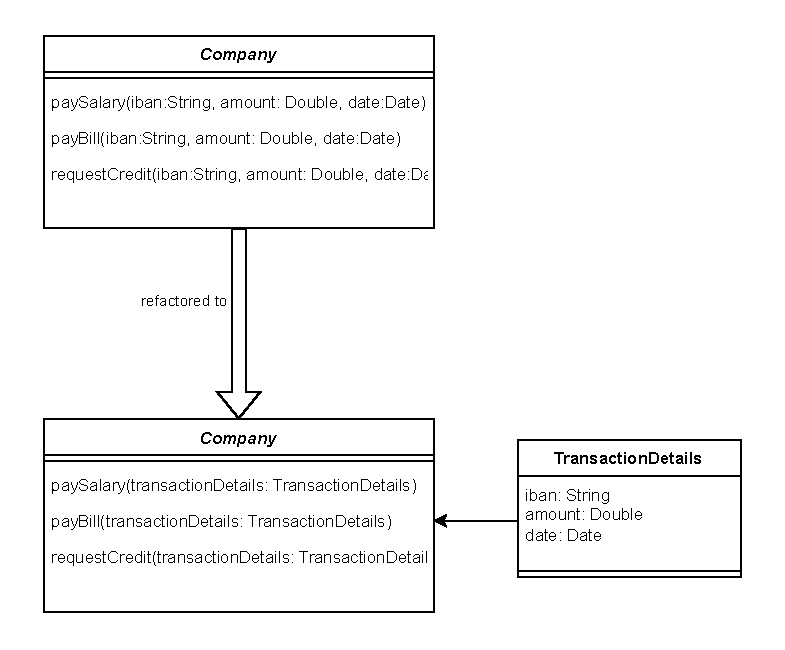
\includegraphics[scale=0.9]{figures/chapter2/dataClump/refactor_simple_case.pdf}
    \caption{A simple data clump and a proposed refactoring}
    \label{fig:company_bill_tax}
\end{figure}
Figure \ref{fig:company_bill_tax} depicts as an UML-diagram a parameters-to-*parameters data clump. The class \textit{Company} has two methods dealing with financial payments. Both methods  receives three parameters, namely an IBAN, a monetary amount, and a transaction date. While this example is comparably small, there could be more classes and methods in a real-world application that receives these three parameters to perform financial operations. As a result, changing the method signature can be time-consuming. For instance, adding a description to a transaction requires changing all affected method signatures and their associated calls. Also changing the datatype of the monetary value (e.~g. a custom Money class) requires similar changes. Additionally, the readability of these methods might be not ideal as a reader would not know what a \textit{IBAN} is or what currency \textit{amount} represents. These facts must be outlined in the documentation which therefore needs to be duplicated for each method. 
 
\subsection{Identifying data clumps}\label{sec:data_clump_detection}

The difficulty of identifying data clumps can vary strongly dependent of how many files are affected by a data clump. If a data clump resides in only one file (e.~g. many methods in the same file share parameter), a trained eye can spot them and apply the necessary refactoring. This \textbf{manual approach} requires however that the developer is willing to spend time detecting a data clump and removing it. 

In contrast, an algorithmic method for finding can be defined as follows:
\begin{figure}
\begin{lstlisting}[numbers=left]
    holders := all potential data clump holders 
            with at least three items inside the project
     For each (h1, h2) in HolderList with h1 != h2
        common := intersection(h1, h2)
        if common.size>=3:
            reportDataClump(h1, h2, common)
        

\end{lstlisting}
\caption{Algorithm for detecting data clumps}
\label{lst:data_clumps_algo}
\end{figure}

In contrast to local code smells like large methods or missing documentation, data clumps can be classified as a global code smell. Considering only a small area of the source code is often not enough because they can be spread over multiple classes and methods. 





Listing \ref{lst:data_clumps_algo} shows how an algorithm to find data clumps could be designed. In the first step all data clump holders must be identified.
A data clump holder is a class that has at least 3 fields or a method that has at least 3 parameters.  Only methods and classed for which source code is available should be detected because refactoring would be impossible otherwise. In case of methods, overridden methods should only be refactored if their super methods also constitutes a data clump that can be refactored.  For instance, if a method overrides another method of which the source code is not available (external library), refactoring would be infeasible. 
It should be noted that other programming languages like C++ can have other data clump holder (e.~g. global variables in namespaces). 


Afterwards, all distinct tuples of data clump holders are compared. If two data clump holders share at least $n$ fields/parameters, they form a data clump which can be reported. Determining common variables require comparing the identifiers and types of the variables and determining whether they are similar as specified in section \ref{sec:data_clump_def}. However, finding common parameters between two data clump holders is not trivial.  For instance, the algorithm does not specify how the identifiers of two data clump holders are compared (strict equality, synonyms). A similar issue arises with the types of the variables.  Two identical type identifiers might refer to different types. Therefore, the type names must be qualified so that they are unique. These details can be crucial for performance optimization and accuracy of its result. 



If a data clump is detected, it can be reported for further processing. For instance, a warning could be displayed in an \ac{IDE} or the detected data clumps can be stored to a file. Here also, the concrete implementation is dependent on how the data clumps will be processed later.

This algorithm has some drawbacks. It has a time complexity of $\Theta(n^2)$ where $n$ is the number of potential data clump holders. Therefore, analyzing  large projects can be time-consuming unless the set of potential data clump holders is reduced beforehand. Nevertheless, it accurately finds every data clump and is deterministic.

In contrast, probabilistic methods use an artificial intelligence like a Large Language Model to detect data clumps. Theses are non-deterministic and their reasoning are not always explainable. However,  these key difference help them to find data clumps that are difficult to find with the algorithmic approach. For instance, they can use synonyms for comparing variable names. 
  
\subsection{Refactoring data clumps}\label{sec:data_clump_refactor}

There are several approaches for refactoring data clumps. The general approach is always feasible and suggested by Fowler.
He outlines two  steps to refactor a data clump:

In the  \textbf{Extract-Class}-step, a class with fields for each data clump item is extracted. A class for this purpose might already exist so that it can be re-used.

In the second step, \textbf{Preserve Whole Object} or \textbf{Introduce Parameter Object} might be applied. This means that the method's signature is changed so that the extracted class replaces the data clump items, and all references to the method are changed accordingly.

If the extracted class already exists, it can be challenging to identify such a class. Given a current refactoring process (i.~e. a bot or human being is currently refactoring data clumps), two possibilities can occur. Either it was created during the ongoing refactoring process so that its location and name is known, or such knowledge is missing. The former case is easy to handle.  The latter variant occurs if the extracted class is created after the data clump is introduced but the data clump is not fixed immediately or the extracted class already existed but for some reasons the data clump was introduced. In this case, a suitable extracted class must be identified which requires extensive knowledge of the source code.

Additionally, there could be classes that are a superset of the required fields to refactor the data clump. Suppose a data clump \textit{x}, \textit{y}, \textit{z} needs to be refactored. There could be a  class \textit{Vector4D} which has the fields  \textit{x}, \textit{y}, \textit{z}, \textit{w}. One could argue that this extracted class could be used by setting \textit{w} to 0 or some other default value. On the contrary, a 4D vector has different application than a 3D vector so that creating a 3D vector class might be more suitable. 

Another approach for refactoring data clumps is applicable to parameters-to-parameters data clumps in the same class. In this case, the parameters can be extracted to fields and removed from the method signature. This approach only works if the values of the parameters are known when creating instances of the class containing the method. It might also create a temporal  coupling if the fields are modified during the execution of the method, which should be avoided. 


In the case of fields-to-fields data clump, introducing a common base class or interface could also help to solve the data clump issue. The new base class contains all data clump items a fields and is inherited by the two classes. Assuming only single inheritance hierarchies are supported, this does not work if at least one class already inherits from another class. In this case, using interfaces instead of classes can partially solve the data clump issue, but the data clump fields still need to be defined for each class.





\subsection{Reasons not to refactor data clumps}\label{sec:data_clump_not_refactor}
While data clumps are a code smell they might not be worth to refactor. 

One reason for not refactoring data clumps is the tendency of producing data classes. These are classes that only provide access to data but no functionality. By extracting a class as outlined in \ref{sec:data_clump_refactor} the new class has no or scarce additional functionality. These data classes can be also seen as a code smell so that refactoring might not reduce the number of code smells significantly. One way to mitigate this risk can be to further refactor the code by moving functionality related to the extracted class to such class thereby preventing data classes \cite{fowler2019refactoring}. 

Another problem is the creation of those data classes is object instantiation. Suppose a method previously requires three parameters \textit{x}, \textit{y}, and \textit{z}. By refactoring the method, it requires only one parameter of a data class (e.~g. \textit{Point}). Callers of such method have previously provided three arguments, and now have to create an instance of \textit{Point}. As a result, many instances can be created that consume memory and require garbage collection resulting in performance loss. While these effects might be minimal, the effect is more significant on embedded systems or other systems with few resources. A similar problem occurs if the access to variables is replaced by getters or setters which also creates some overhead. While many compilers are capable of optimizing such issues, they should nevertheless be considered. 

Also over-engineering can be an issue. As noted in \ref{sec:data_clump_def}, one can check the existence of a data clump by testing whether the removal of one parameter would make sense. This however is arbitrarily and no concise criteria can be given. Sometimes a group of parameters are connected but an extracted class would create a layer of abstraction that is unnecessary and makes the code even harder to read. This is particular important if the domain of each of the three variables is so distinctive that a common class name is hard to find.

In modular software projects, extracting a class can cause unwanted or even impossible dependencies.  Suppose a software project has a component for server-related code and for client-related code. Neither of this code is dependent of the other (i.~e. classes in one component are not visible in the other). A data clump connecting those components can only be refactored if the extracted class is located somewhere else. For instance, one could create a \textit{util} package. However, this creates an indirect dependency between server and client code and also might overload the \textit{util} package because it should not contain domain-specific code. 

\begin{comment}
	Inhalt...

\subsection{Representation of data clumps}\label{sec:data_clump_graph}

Data clumps can be represented as a graph, so that clusters or pattern can be detected to further evaluate whether a specific data clump is worth refactoring. 

For instance, a graph can be constructed that contains nodes for each class and additionally each method in the software project. If two methods form a data clump, they are connected by an edge in the graph representation. Similarly, two classes connected by an edge if there is a data clump relationship, or a class and a method   

Another approach is proposed by Baumgartner et al. Here, only the classes that contain data clumps are represented as nodes, and two nodes are connected by an edge if there is a data clump relationship between those two classes. For instance, an edge exists if a method in one class and another method in a separate class are part of a parameters-to-parameters data clump. \cite{data_clumps_baumgartner}.


To discern one data clump from another, a \textbf{types-names-identifier} is used in this master thesis. This identifier is created by sorting the data clump items by identifier, then joining the data type and identifier of each data clump with a white space, and concatenating these strings with a semicolon. For instance given a data clump \textit{boolean sign}, \textit{int exponent}, and \textit{double mantissa}. The respective types-names-identifier is \textit{int exponent;double mantissa;boolean sign}. This key identifies a data clump based on its types and names thereby helping to find related data clumps. 



One approach to represent and serialize data clumps for reporting purposes is the \textbf{Data clumps Type Context} \cite{dataclump_type_context} developed by Baumgartner et al. Each data clump is described by the affected files, classes and methods (if applicable). Additional, the precise location of each data clump is given Hence,  it employs the first graph representation mentioned in this section meaning that individual classes and methods are forming the data clump graph. However, the second variant can be re-constructed as well using this information. 
A full description of the format can be found in appendix \ref{sec:data_clump_format}

\end{comment}


